% !TeX root = ../../main.tex
\section{Detailed capital cost breakdown}
\subsection{Equipment cost}
Purchase cost of equipment is obtained from different resources. Towler \cite{sinnott_chemical_2020} has proposed the following correlation to calculate the buying price in year 2006.
\begin{equation}
    C_{e}=\ a+bS^n
\end{equation}
Where, a, b and n are constants depending on the equipment type and S is the key costing parameter of the equipment. Matche \cite{noauthor_matches_nodate} gives the price in year 2014 and Douglas \cite{douglas_conceptual_1988} provides the method for calculating cost in mid-1968. After applying a location factor and cost escalation factor, an average price from the three sources is taken to be the purchased price. However, as Nitroma employed new technologies such as suspension melt crystallisation, price for a few units cannot be extrapolated from cost correlations. In this case, similar unit price from different suppliers is compared and approximations are made where necessary. For the purpose of reducing corrosion, 316 stainless steel has been identified as the material for majority of equipment.

\begin{table}[H]
\centering
\caption{Equipment purchase cost}
\label{tab:equipment purchase}
\begin{tabular}{llS[table-format=7.2,round-mode=figures,round-precision=3]}
\toprule
\textbf{Equipment Type}    & \textbf{Number of Equipments} & \textbf{Purchase Cost (\$)} \\\midrule
Heat Exchangers            & 20                            & 143784.99                  \\
Electric Heaters           & 13                            & 640728.64                  \\
Reactors                   & 6                             & 271879.49                  \\
Packed Columns             & 10                            & 99443.17                   \\
Flash Vessels              & 3                             & 2305.55                    \\
Gravitational Decanters    & 1                             & 4493.06                    \\
Crystallizer               & 2                             & 42503.76                   \\
Wash column                & 1                             & 16668.24                   \\
Refregiration system       & 2                             & 37935.77                   \\
Storage (Buffer) Tanks     & 12                            & 879434.57                  \\
Mixers                     & 5                             & 82320.88                   \\
Pumps                      & 10                            & 47430.51                   \\
Fan                        & 4                             & 33157.33                   \\
Granualtor                 & 2                             & 49241.20                   \\
Waste Treatment Equipments & 3                             & 50978.91                   \\ \midrule
\textbf{Total}             & 94                            & 2402306.05                 \\ \bottomrule
\end{tabular}
\end{table}

\Cref{tab:equipment purchase} summarized all major units purchased by Nitroma. Due to the variety of equipment types, detail breakdown of individual equipment cost is not discussed here but can be found in \cref{app:capexbreakdown}.

The inside battery limits (ISBL) investment is the cost of purchasing and installing all equipment. Lang has proposed ISBL is a function of the installation factor and the purchase cost calculated above.
\begin{equation}
    ISBL=F\sum C_{e}    
\end{equation}
As both solids and fluids are processed in Nitroma's plant, the installation factor is 3.63, leading to an ISBL value of \$8.72 million. However, Towler \cite{sinnott_chemical_2020} has introduced a factorial method with individual installation factors:
\begin{equation}
    ISBL=\sum C_{e}\left(1+f_{p}+\frac{f_{er}+f_{el}+f_{i}+f_{c}+f_{s}+f_{l}}{f_{m}}\right)
\end{equation}
Values of each installation factor can be found in \textbf{Appendix}. Using this method, the overall installation factor is calculated to be 3.68 and ISBL is \$8.84 million.

\subsection{Additional capital costs}

\begin{table}[H]
\centering
\caption{Additional CAPEX cost}
\label{tab:CAPEXadditional}
\begin{tabular}{llS[table-format=7.0]}
\toprule
\textbf{Item}        & \textbf{Description }                                                                      & \textbf{Cost (\$)}       \\\midrule
OSBL        & Outside Battery Limits, this is cost that is addition to the                      & 3536195 \\
            & equipment cost and accounts for site infrastructure. OSBL                         &           \\
            & is estimated to be \SI{40}{\percent} of ISBL.                                                  &           \\\midrule
Land        & Industial land price is \$24.33/m\textsuperscript{2} in Nanjing. & 2920000 \\
            & Plant size is 0.12km\textsuperscript{2}.                         &           \\\midrule
Design \&   & Cost spent designing and constructing the plant, typically paid to                & 3094170 \\
Engineering & contractor. This is approximately \SI{25}{\percent} of the sum of ISBL and OSBL.               &           \\\midrule
Contingency & Extra costs added to the project to allow fluctuation of the                      & 1237668 \\
            & cost estimate since the number of equipments is uncertain                         &           \\
            & until the construction phase. Approximated to \SI{10}{\percent}                             &           \\
            & of the sum of ISBL and OSBL                                                       &           \\\midrule
One-off     & The plant has installed a refrigeration cycle to lower the                        & 9315     \\
chemicals   & operating temperature of one of the crystallizers. Given                          &           \\
            & that the refrigerant does not need to be replaced,                                &           \\
            & it is categorized as CAPEX.                                                       &           \\\midrule
Working     & Funds to purchase raw materials, catalysts and utitlies for start-up              & 2944278 \\
Captial     & prior to earning profit.                                                                    &       \\\bottomrule   
\end{tabular}
\end{table}

\subsection{CAPEX summary}
\begin{wrapfigure}{r}{8cm}
    \vspace{-1.1cm}
    \label{fig:CAPEXSummary}
    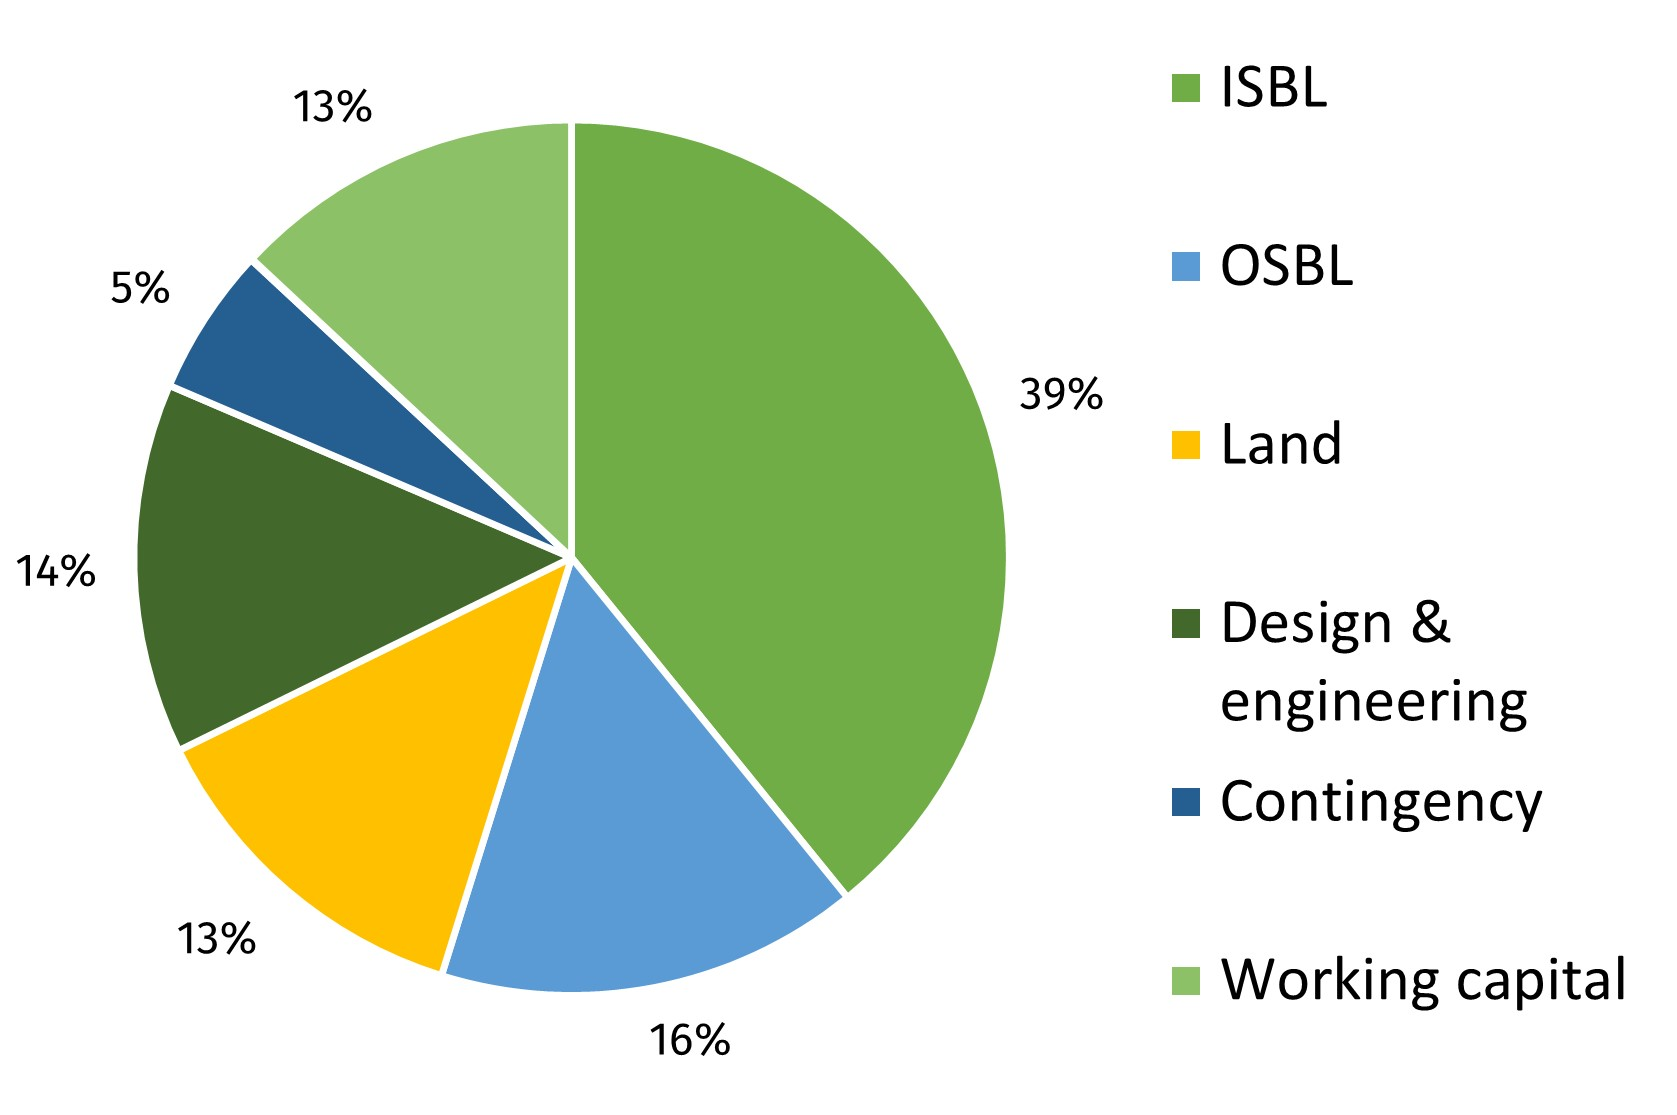
\includegraphics[width=0.42\textwidth]{chapters/6-economics/figures/CAPEX_summary.jpg}
    \caption{CAPEX Summary}
\end{wrapfigure}
Total investment of Nitroma was calculated to be \$22.6 million, by adding ISBL and additional costs listed in Table \ref{tab:CAPEXadditional}. It should be noted that since Nitroma is operating as a small-scale plant, separation units, particularly packed columns, are smaller than common industrial-installed units. This contributed to the low investment figure.
\vspace{5cm}